\documentclass[20pt,landscape,pdftex]{foils}

\usepackage{./ppftlk}
\renewcommand{\P}{\text{P}}
\newcommand{\MC}{\multicolumn}
\renewcommand\r{\right}
\renewcommand\l{\left}
\newcommand\dist{\buildrel\rm d\over\sim}
\newcommand\ind{\stackrel{\rm indep.}{\sim}}
\newcommand{\cY}{{\cal Y}}
\newcommand{\cT}{{\cal T}}
\setlength{\doublerulesep}{\arrayrulewidth}
\newtheorem{assumption}{Assumption}
\newcommand{\indep}{{\bot\negthickspace\negthickspace\bot}} 
\newcommand\spacingset[1]{\renewcommand{\baselinestretch}%
{#1}\small\normalsize}

%
\title{Matching as Nonparametric Preprocessing for Improving
  Parametric Causal Inference}

\date{September 2, 2004}
\author{Daniel E. Ho \\
  Yale Law School\\
  \\
  Kosuke Imai\\
  Department of Politics\\ Princeton University \\
  \\ 
  Gary King\\
  Department of Government\\ Harvard University\\
  \\
  Elizabeth A. Stuart\\
  Department of Statistics\\ Harvard University
\mbox{}\pdfbookmark{TitlePage}{stlab0}}

\parindent=0pt
\begin{document}
\color{black}
\LOGOOFF
%\hypersetup{pdfpagetransition={Split /Dm /H /M /O}}
%\hypersetup{pdfpagetransition={Blinds /Dm /H}}
\hypersetup{pdfpagetransition={Box /M /O}}
%\hypersetup{pdfpagetransition==Dissolve}
\maketitle

%%%%%%%%%%%%%%%%%%%%%%%%%%%%%%%%%%%%%%%%%%%%%%%%%%%%%%%%%%%%%%%%%%%%%%%%%%%%%%%

\foilhead{The Problem: Model Sensitivity\pause}

\hypersetup{pdfpagetransition=Replace}

\begin{itemize}
\item Most political scientists use a parametric model (e.g., linear
  regression).\pause
  \begin{itemize}
  \item select one model specification from many possible
    specifications.\pause
  \item assume the selected model is correct without such
    knowledge.\pause
  \item ``correct'' specification is chosen after looking at the
    estimates.\pause  
  \item present several {\it selected} specifications to show your
    results are ``robust.''\pause
  \end{itemize}

\item To readers of an article\pause 
  \begin{itemize}
  \item it's never clear whether it represents a true test of an ex
    ante hypothesis.\pause
  \item or whether it merely shows it's possible to find such
    results.\pause
  \end{itemize}
  
\item Statistics textbooks do not tell us what to do.\pause
  
\item Our idea: reduce model dependence without introducing
  bias.\pause
  \begin{itemize}
  \item preprocess the data without looking at the estimates.\pause
  \item run the same parametric model on the preprocessed data.\pause
  \end{itemize} 
\end{itemize}


%%%%%%%%%%%%%%%%%%%%%%%%%%%%%%%%%%%%%%%%%%%%%%%%%%%%%%%%%%%%%%%%%%%%%%%%%%%%%%%

\foilhead{Introduction\pause}

\hypersetup{pdfpagetransition=Replace}

\begin{itemize}
\item Matching, a new statistics literature on causal inference:\pause
  \begin{enumerate}
  \item nonparametric, non-model based methods.\pause
  \item reducing or eliminating functional form and other assumptions.\pause
  \end{enumerate}
  
\item But, from the point of view of practical researchers,\pause
  \begin{enumerate}    
  \item conflicting techniques, practices, guidelines, and rules of thumbs. \pause
  \item calculation of valid standard errors is complicated or
    unavailable.\pause
  \item few theoretical results.\pause
  \end{enumerate}

\item Our unifying idea of this diverse literature:\pause 
  \begin{enumerate}
  \item use matching NOT as a substitute for familiar parametric
    regression analysis.\pause
  \item use matching to make conventional parametric models work better.\pause
  \end{enumerate}

\item Under our proposed framework,\pause
  \begin{enumerate}
  \item parametric analyses are applied to preprocessed data rather
    than to raw data.\pause
  \item valid standard errors are readily available.\pause
  \item resulting estimates are less model dependent.\pause
  \end{enumerate} 

\item Easy-to-use software: MatchIt available at
  http://gking.harvard.edu/matchit/\pause
\end{itemize}

%%%%%%%%%%%%%%%%%%%%%%%%%%%%%%%%%%%%%%%%%%%%%%%%%%%%%%%%%%%%%%%%%%%%%%%%%%%%%%%

\foilhead{Definition of Causal Effects\pause}

\hypersetup{pdfpagetransition=Replace}

\begin{itemize}

\item Example: estimating the electoral advantage of incumbency for
  Democrats\pause
  \begin{itemize}
  \item Units: congressional districts, $i=1,\dots,n$.\pause
  \item Observed treatment: Democratic incumbent ran $(t_i=1)$, did
    not run $(t_i=0)$.\pause
  \item Observed outcome: Democratic vote share for the $i$th
    district, $y_i$.\pause
  \item Control variables: use pretreatment variables $X_i$ and avoid
    posttreatment bias.
  \end{itemize}

\item Potential outcomes: $y_i(1) \equiv y_i(t_i=1)$ and $y_i(0)
  \equiv y_i(t_i=0)$\pause  
  \begin{itemize}
  \item Realized Causal Effect for unit $i$: $y_i(1) - y_i(0)$.\pause
  \item The fundamental problem of causal inference.\pause
  \item Connection to missing data and ecological inference:\\ $y_i =
    t_i y_i(1) + (1-t_i) y_i(0)$\pause
  \item Random causal effect for unit $i$: $Y_i(1) - Y_i(0).$\pause
  \item Mean causal effect for unit $i$: $E[Y_i(1) - Y_i(0)].$\pause
  \end{itemize}

\item Quantities of interest:\pause
  \begin{itemize}
    \item Average Treatment Effect: $ATE = \frac{1}{n}\sum_{i=1}^n
      E[Y_i(1) - Y_i(0)]$\pause 
      \bigskip
    \item Average Treatment Effect for the Treated:\\ ATT =
      $\frac{1}{\sum_{i=1}^n t_i}\sum_{i:t_i=1} E[Y_i(1) -
      Y_i(0)]$\pause 
  \end{itemize}
\end{itemize}

%%%%%%%%%%%%%%%%%%%%%%%%%%%%%%%%%%%%%%%%%%%%%%%%%%%%%%%%%%%%%%%%%%%%%%%%%%%%%%%

\foilhead{Data Collection Mechanisms\pause}

\hypersetup{pdfpagetransition=Replace}

\begin{itemize}
\item Key features of classical randomized experiments:\pause
  \begin{enumerate}
  \item random selection of units from a given population.\pause
  \item random assignment of values of the treatment.\pause
  \item large $n$.\pause
  \end{enumerate}
\item Observational studies:\pause
  \begin{itemize}
  \item do not meet all three features of classical randomized
    experiments\pause
  \item comprise almost all political science research
  \end{itemize}

\item Assumptions for causal inference:\pause
  \begin{itemize}
  \item no sample selection bias.\pause
  \item no omitted variable bias.\pause
  \item no posttreatment bias.\pause
  \item independent units.\pause
  \item same treatment within each treatment group.\pause
  \end{itemize}
\end{itemize}

%%%%%%%%%%%%%%%%%%%%%%%%%%%%%%%%%%%%%%%%%%%%%%%%%%%%%%%%%%%%%%%%%%%%%%%%%%%%%%%

\foilhead{Parametric Analysis Methods\pause}

\hypersetup{pdfpagetransition=Replace}

\begin{itemize}
\zerolistvertdimens 
\item Researchers typically assume a parametric model (up to unknown
  parameters):\\ e.g., $Y_i \sim p(\mu_i, \theta)$ with $\mu_i \equiv
  E(Y_i \mid t_i, X_i)=g(\alpha+t_i \beta + X_i \gamma)$\pause
\item but, the true model is unknown.\pause
\item In experimental studies, $T$ and $X$ are independent and so $X$
  can be dropped:\pause 
  \begin{itemize}
  \item $ATT = g(\alpha+\beta) - g(\alpha).$\pause
  \item The results do not depend on the functional form,
    $g(\cdot)$.\pause 
  \end{itemize}
\item In observational studies, the results are model-dependent.\pause
  \begin{itemize}
  \item curse of dimensionality: $m$ 10-category variables require
    $10^m$ parameters in regression.\pause
  \end{itemize}
\end{itemize}

 \begin{center}
   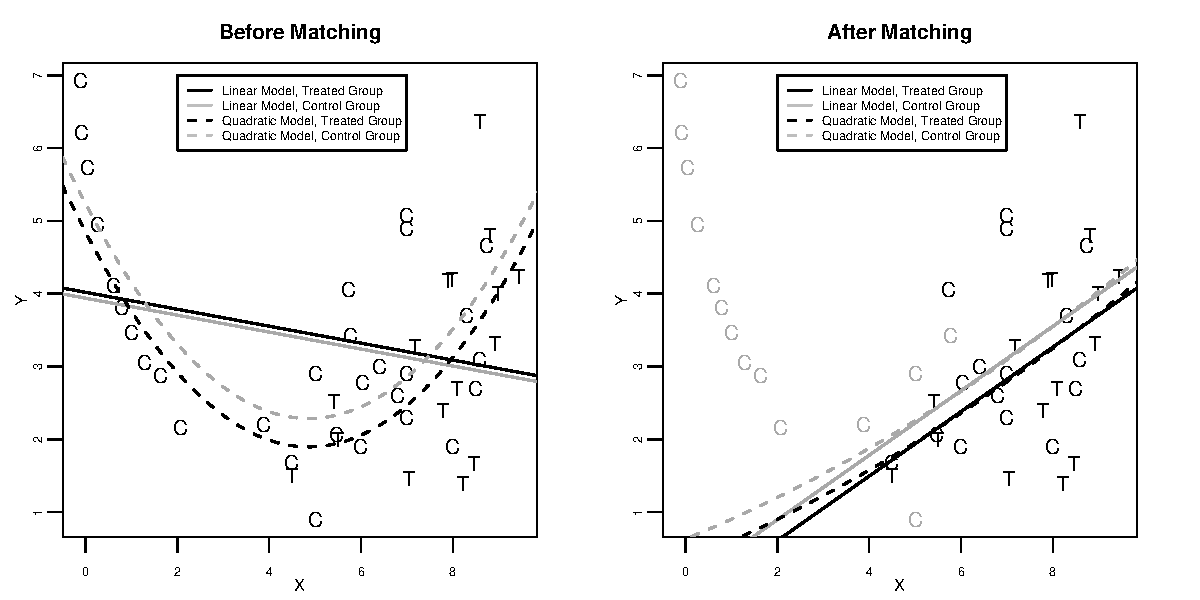
\includegraphics{figs/olspanel-thick.pdf}\pause
 \end{center}

%%%%%%%%%%%%%%%%%%%%%%%%%%%%%%%%%%%%%%%%%%%%%%%%%%%%%%%%%%%%%%%%%%%%%%%%%%%%%%%

\foilhead{Nonparametric Preprocessing\pause}

\hypersetup{pdfpagetransition=Replace}

\begin{itemize}
\item Adjust the data prior to the parametric analysis so that:\pause
  \begin{enumerate}
  \item the relationship between $t_i$ and $X_i$ is eliminated or reduced.\pause
  \item no bias and little inefficiency is induced.\pause
  \end{enumerate}

\item Fundamental rule for avoiding selection bias: do not select on
  dependent variable.\pause 
  \begin{itemize}
  \item valid selection rule -- a function of $t_i$ and $X_i$.\pause 
  \item randomized blocks in experiments, stratified sampling in
    surveys.\pause
  \end{itemize}

\item Preprocessed data set\pause
  \begin{itemize}
  \item contains a subset of the raw data.\pause
  \item $p(X\mid t_i=1) = p(X\mid t_i=0)$ for one-to-one exact
    matching.\pause
  \item $p(X\mid t_i=1) \approx p(X\mid t_i=0)$ for nonexact matching
    methods.\pause 
  \item model-dependence is reduced.\pause
  \end{itemize}
\end{itemize}

%%%%%%%%%%%%%%%%%%%%%%%%%%%%%%%%%%%%%%%%%%%%%%%%%%%%%%%%%%%%%%%%%%%%%%%%%%%%%%%

\foilhead{Choosing a Matching Procedure\pause}

\hypersetup{pdfpagetransition=Replace}

\begin{itemize}
\zerolistvertdimens 
\item The goal of matching: improve balance without losing too many
  observations.\pause

\item Try different matching procedures until better balance is
  achieved.\pause

\item But, do not examine the outcome variable during
  preprocessing.\pause
\end{itemize}
  
\begin{enumerate}
\item Select Covariates: include all variables that would have been
  included in the parametric model, but avoid posttreatment
  bias.\pause
  
\item Try Exact Matching: if a large number of units are matched, go
  to the parametric analysis.\pause
  
\item Use Propensity Score Matching: summarize all the variables in
  $X$ with a single variable, $e_i(X_i)=\Pr(t_i=1\mid X_i)$.\pause
  
  \begin{enumerate}
  \item propensity score tautology: it works when it works, and when
    it doesn't work, it doesn't work.\pause

  \item logistic regression, GAM, CART, neural network, etc.\pause
    
  \end{enumerate}

\item Evaluate the Matching Procedure: look at various low-dimensional
  summaries of $X$.\pause
\item Parametric Outcome Analysis: same method, same algorithm, same
  software, same model checking procedures, ... \pause
\end{enumerate}

%%%%%%%%%%%%%%%%%%%%%%%%%%%%%%%%%%%%%%%%%%%%%%%%%%%%%%%%%%%%%%%%%%%%%%%%%%%%%%%

\foilhead{Empirical Illustration\pause}

\hypersetup{pdfpagetransition=Replace}

\begin{itemize}
\item Democratic senate majorities and FDA drug approval time
  (Carpenter 2002).\pause
  \begin{itemize}
  \item Hypothesis: ``expected approval times are greater when
    Democrats control the White House, when the agency's oversight
    committees are more liberal, and when the House and Senate are
    more liberal'' (p.495).\pause
  \item liberal FDA oversight should lead to slower approval of new
    drugs.\pause 
  \end{itemize}

\item Original analysis:\pause
  \begin{itemize}
  \item 408 new drugs (262 approved, 146 pending).\pause
  \item lognormal survival model.\pause
  \item seven oversight variables (median adjusted ADA scores for
    House and Senate Committees as well as for House and Senate
    floors, Democratic Majority in House and Senate, and Democratic
    Presidency).\pause
  \item 18 control variables (clinical factors, firm characteristics,
    media variables, etc.)\pause
  \end{itemize}

\item Our analysis:\pause
  \begin{itemize}
  \item focuses on the causal effect of a Democratic majority in the
    Senate.\pause
  \item omits variables that are highly likely to be affected by the
    treatment.\pause
  \item uses one-to-one nearest neighbor propensity score matching.\pause
  \item discards 49 units (2 treated and 17 control units).\pause
  \item runs 262,143 possible specifications and calculates ATE.\pause
  \end{itemize}
\end{itemize}

%%%%%%%%%%%%%%%%%%%%%%%%%%%%%%%%%%%%%%%%%%%%%%%%%%%%%%%%%%%%%%%%%%%%%%%%%%%%%%%

\foilhead{Improved Balance and Reduced Model Dependence\pause}

\hypersetup{pdfpagetransition=Replace}

\begin{center}
  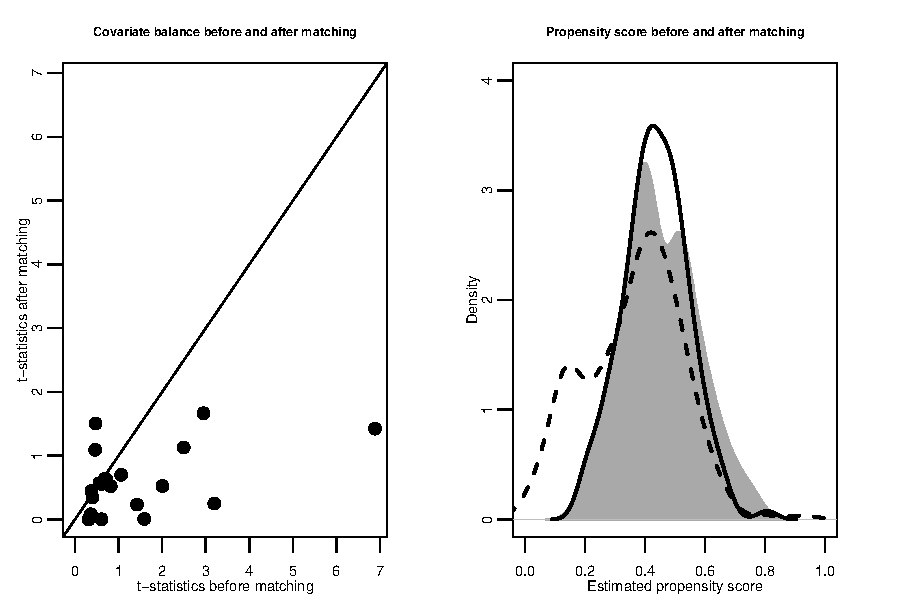
\includegraphics[scale=1.2]{figs/fdabal}\pause \\
  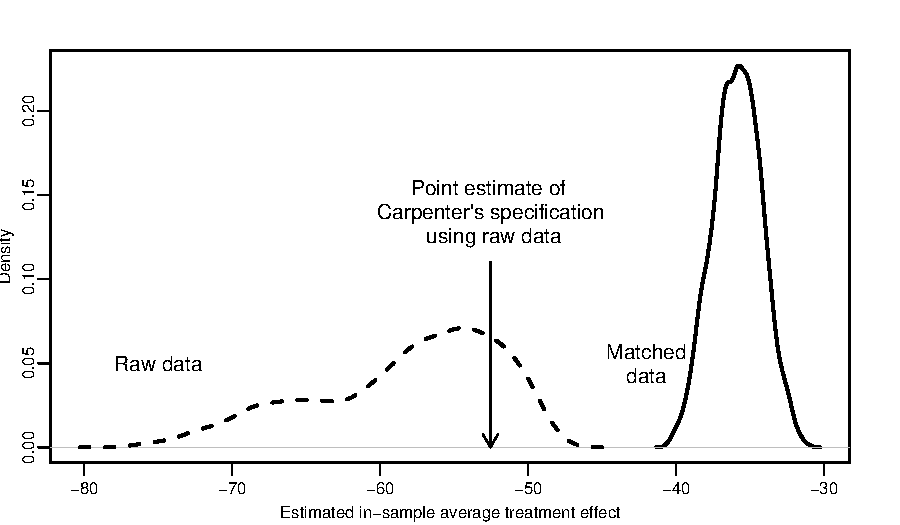
\includegraphics[scale=1.2]{figs/fdadens}\pause
\end{center}

%%%%%%%%%%%%%%%%%%%%%%%%%%%%%%%%%%%%%%%%%%%%%%%%%%%%%%%%%%%%%%%%%%%%%%%%%%%%%%%

\foilhead{Concluding Remarks\pause}

\hypersetup{pdfpagetransition=Replace}

\begin{itemize}
\item What can go wrong\pause
  \begin{itemize}
  \item curse of dimensionality in balance diagnostics.\pause
  \item preprocessing data may increase variance while reducing
    bias.\pause 
  \item change in quantities of interest.\pause
  \end{itemize}
\item We provide a way to get around the ethical and methodological
  problem of choosing a model specification.\pause
\item Preprocessing the raw data with matching procedures makes
  familiar parametric models a much more reliable tool.\pause

\item Preprocessing makes causal inference less sensitive to modeling
  assumptions.\pause 
\end{itemize}


\end{document}
